\chapter{Background}


This thesis is an exploration of the methods in adaptive sampling for marine robots. The work has kept the scientific goal in mind, while applying adaptive strategies for data collection, increasing the scientific value. In order to properly introduce the multi disciplinary field of adaptive sampling with marine robots, a host of concepts and background needs to be introduced. This chapter briefly introduces the environment, the ocean, how to sense it and its possibilities and constraints on the robot, the robots themselves with their capabilities and constraints.


\section{The Ocean}
The ocean is in constant flux; tides, weather, currents, seasons, and climate change, they all contribute to the fluid state of our oceans. Information in the ocean is heterogeneous and unevenly distributed, while vast areas can be virtually the same water, other areas can exhibit extreme gradients and temporal changes. The opposite can also be true, where the only thing changing is measurable in time, not space. The ocean changes both in time \textit{and} space, or \textit{spatio-temporally}, from the tiniest turbulence to the largest 1000s-year current cycles of Milankovitch thermohaline circulation \cite{talley2011descriptive}, it is always in flux. An extensive listing of ocean phenomena suited for adaptive sampling is presented in Hwang \cite{hwang2019auv}. Measuring ocean parameters thus becomes trying to hit a moving target, and thus, the right tool is required.

\subsection*{Oceanography}
Physical oceanography is a sub-field of geophysics, and the study of all aspects of the physical ocean, founded at the time of the Challenger expedition \cite{thomson1873challenger} (1872-1876). Currents, densities, tides, temperatures, waves, turbulence and their interactions with each other and their boundaries (atmosphere, ice, and seabed) is the main concern of oceanography. Their main tools are the \acrfull{ctd}, the \acrfull{adcp} and the turbulence probe. These sensors, mounted on ships, rigs and robots, provide the data necessary to estimate heat fluxes to the arctic from the Gulf stream, project the salinity outside Galapagos and estimate the rate of warming in the Eastern Barents Sea.  

\begin{figure}
    \centering
    \includegraphics[width=\textwidth]{figures/challenger.png}
    \caption{Track of H.M.S. Challenger December 1872 to May 1876 showing the dredging an trawling stations and the ocean density in the surface. Densities from observations made on board the H.M.S. Challenger and other vessels. Engraved by Malby \& Sons. }
    \label{fig:challenger}
\end{figure}

\subsubsection*{Oceanography - Stratification}
A key finding of oceanography is that the ocean is \textit{flat}, that is, the vertical variability is greater than the horizontal \cite{talley2011descriptive}. This effect has affected oceanography by shaping its primary mode of sampling: vertical profiling. In vertical sampling, the term \textit{water column} arises, and is defined as the column of water between the surface and the \textit{benthos}, or seabed. The ocean is often found to be \textit{stratified}, or layered. If the vertical density gradient is non-negative in the entire water column, the water column is \textit{stable}. This means that the denser water is below the less dense, and mixing of the water is dependent on some external force, such as wind or current. The opposite is also true, that an \textit{unstable} water column is possible, inducing a vertical motion and mixing. Just as waves can occur at the air-water interface, they can occur in stratified layers, creating internal waves. These generally have  larger wavelengths, amplitudes, and periods, due to the forcing being weaker between two ocean strata, than between the ocean and air. 

\subsubsection*{Oceanography - Upwelling}
When wind blows over the sea surface, the water is accelerated and advected along with the wind, as this force propagates through the water column, through shear forcing a rotation occurs. This is caused by the Coriolis-effect, and results in a net transport of water perpendicular to the wind direction, known as the Ekman spiral \cite{ekman1902om}. This again means that when the wind is blowing from the North on a Western shoreline in the Norhtern hemisphere, water will be advected away from the shore. This leads to \textit{upwelling}, in which the advected water is replaced by the deeper water in the surrounding area. 

\subsubsection*{Oceanography - Fronts}
Ocean fronts, named after war time fronts, are where water masses with different characteristics meet \cite{talley2011descriptive}. As their namesake, fronts are fairly static in location, and they are characterized by sharp horizontal gradients  in relation to the ocean at large. The polar front in the Barents Sea, where the Atlantic meets the Arctic ocean, there is a strong temperature gradient along the North-south axis. At estuaries, river plumes and fronts occur as salinity gradients, and depending on the difference in river and ocean temperature, temperature gradients. If there is little or no forcing from wind, currents, and waves, the river front tends to float atop the ocean as a fresher layer. Its extent can also be temporally varying with tides, in cases where tidal variation pump water out of the river. 

\subsubsection*{Oceanography - Turbulence}
As the ocean flows, mixes, and settles, it generates turbulence, or tiny fluctuations in salt, temperature, and momentum. My measuring such fluctuations, oceanographers are able to estimate the \textit{dissipation rate}, or the rate at which the kinetic energy of the ocean is dissipated to heat via viscous friction. 
\begin{quote}
    Quantifying the magnitude and
distribution of the dissipation rate helps identify the different forcing mechanisms and their relative contribution in mixing. \\
 - \textcite{kolas_technical_2021}
\end{quote}

Additionally, phenomenon such as Langmuir circulation, eddies,  tides, Ekman layers and polynyas \cite{talley2011descriptive} complicate the picture of the homogeneous ocean, and make for relevant targets of adaptive sampling. 

\subsection*{Marine biology}
The ocean hosts the smallest viruses and bactera, alongside the largest mammals ever to inhabit the earth, the blue whale, \textit{Balaenoptera musculus}. It is the largest and most diverse habitat, from the Arctic to Antarctica, from the light filled surface to the great, dark abyssal planes, spanning this pale blue dot. Long it was considered a black box, humans could not go there, and if you threw something in, it usually did not come back. Today, we are gaining a glimpse of the ocean and its complex ecosystems, one dive, net, trawl, measurement, and echogram at the time, and understanding these ecosystems and how they impact and are impacted by human activity is as critical as ever. While ocean sampling still is parsimonious, 


\section{Sensing}
Of the above phenomena, what can we sense? Measurements and sampling in the ocean can take many forms, from remote sensing to \textit{in-situ} measurements. With remote sensing techniques, mesoscale patterns in the surface come into view, and with \textit{in-situ} sensors, microscales scales of sub-centimeter resolution can be achieved\cite{davies2017use}. 

Sensing can be split into two parts; the acquisition of a measurement and the interpretation of the measurement. Here, both aspects will be explored, starting with measurements made by \textit{in-situ} sensors, continuing to how the signals can be filtered and finishing with the generation of new features from the measurements. For a more complete list of possible oceanic phenomena to sense, see \textcite{hwang2019auv}. Note that the terms \textit{sensing}, \textit{measurement}, and \textit{sampling}. are distinct and separate. With \textit{sensing} being the act of measuring or estimating from measurements a feature of the environment, \textit{measurement} refers to the discrete measurements, or raw data, and \textit{sampling} has two meanings, depending. \textit{Adaptive sampling} is the deliberate taking of a measurement at a certain place and time (from statistics), while \textit{sampling} is the taking of a physical sample (from natural science). 

\subsection{Sensors}
In the oceanic domain, there are many variables to measure, such as temperature, hydrocarbon concentration, and currents. Measurements from \textit{in-situ} sensors can help estimate these variables. It is important to note that in relation to a physical sample, a measurement is more of an indication, and the sample can tell us a lot more. When designing a sensor, from first principles, effects such as thermal expansion, conductivity, and elastic deformation are taken into account. Early thermometers relied on the thermal expansion of mercury for reading the ambient temperature, whereas modern ones can use a host of methods for determining the ambient temperature. In a materiel with high thermal conductivity, such as water, a thermistor can be used. A thermistor is a material in which the resistance varies greatly with temperature. 


\subsubsection*{Conductivity Temperature Depth}
 The most common measurement done by Oceanographers is the triple measurement of \acrfull{ctd}, from these data, the salinity of the ocean can be inferred. The measurements from the \acrshort{ctd} are usually accurate and precise, with little sensor drift. Bias due to physical change in the conductivity cell, such as corrosion, being a larger error-source in the \acrshort{ctd}. The \acrshort{ctd} instrument is usually fixed on a winched rig and used for profile measurements of the ocean. It is also the most common instrument carried by \acrshort{auv}s and gliders. Due to the high accuracy of the instrument and the fact that it is a point measurement that has to be moved through the water column on relatively slow platforms, small fluctuations in the ocean might occur as process noise (Section \ref{sec:noise}). \acrshort{ctd} data was used for adaptive sampling by \textcite{fossum2021adaptive,fossum2021learning,zhang2012autonomous}, in addition to the work presented \textbf{papers A, B, D, E, and F}. 

\subsubsection*{Fluorescence}
Fluorescence sensors work by emitting light at specific wavelengths and measuring the fluoresced, or emitted, light, at a longer wavelength. Elements and molecules that fluoresce absorb some of the energy in the light, and emit the remainder as longer wavelength light, with known photochemical properties. By fluorescence, the amount of chlorophyll a can be inferred, such as in \textcite{kemna2018multi,fossum2019toward} and \textbf{paper C}. Chlorophyll a values can be inferred by emitting light at $470$nm and measuring the emitted light at $695$nm \cite{boss2016primer}. \acrfull{cdom} such as in \textcite{zhang2011peak} can be inferred by emitting light at $370$nm and measuring the emitted light at $460$nm. Further, it is possible to detect uranine at $470/530$nm, phycocyanin at $630/680$nm, and phycoerythrin and rhodamine at $520/595$nm. 

\subsubsection*{Optical properties}
Turbidity and Optical backscatter (indicative of the turbidity), such as in \textcite{berget2018adaptive} can be inferred by measuring the backscattered white light from an optical sensor. These sensors tend to produce more noisy measurements than the CTD. 

\subsubsection*{Echo Sounders}
Echo sounders, or acoustic sensors, are used for seabed mapping, fish and zooplankton tracking, and current measurements depending on their design. Seabed mapping is out of scope for this work, and zooplankton and fish data from an echo sounder is hard to interpret as a measurement. Current mapping could be an avenue of investigation, however, there is no work on this in the literature included in this work. Currents are usually measured by an \acrshort{adcp}, however, the data processing of the \acrshort{adcp} data can be time and labor intensive, making it more difficult to work with as an input for adaptive sampling. There would be great value in developing the capability, since the acoustic instruments measure along the line of travel of a sound wave, thus expanding from point samples to line samples. 

\subsubsection*{Synthetic Features}
It is possible to construct features or measurements from the data collected by sensors, one such feature may be the spatial temperature gradient over a front or the depth of a certain water mass, such as a river plume. In \cite{zhang2016autonomous}, the vertical temperature difference, $\Delta Temp_{vert}$, of each yoyo-profile was used as a measure of the degree of mixing in the water column. They formulated it as in Equation \eqref{eq:sense_tvert}, where $Temp_{depth\_i}$ is the temperature measured at $depth\_i$. 

\begin{align}
    \label{eq:sense_tvert}
    \Delta Temp_{vert} = \frac{1}{N} \sum_{i=1}^N \Big|Temp_{depth\_i}-\Big(\frac{1}{N} \sum_{i=1}^N Temp_{depth\_i} \Big)\Big|
\end{align}

$\Delta Temp_{vert}$ was then used to determine if the AUV was in upwelled (and well mixed) or stratified waters. This points to an important aspect of constructing features; they have to make sense in the context they are used. There are many constructs one could make, but few that would be informative, this imposes the need for oceanographic knowledge in the construction of features. In \textbf{paper A}, the polar front was approximated at the location of the largest horizontal temperature gradient along a transect. Similarly, the river plume depth used as measurements in \textbf{paper B} was constructed by finding the depth of the largest salinity gradient. 



\subsection{Filters}
\subsubsection*{Low-pass filers}
A low-pass filter will smooth out noisy measurements, however if the mean of the underlying signal is moving, the mean of the filtered signal will lag behind. A formulation of the discrete time low-pass filter is presented in Equation (\ref{eq:lowpass}), where $\hat{y}_k$ is the filtered measurement, $y_k$ is the measured (noisy) value, and $\alpha$ is the low-pass weight; increasing it would increase the smoothness. 

\begin{align}
\label{eq:lowpass}
    \hat{y}_i &= \alpha \hat{y}_{i-1} + (1-\alpha)y_i \\
    \alpha &\in [0,1)
\end{align}

One version of this filter has been used \cite{zhang2011peak,zhang2019autonomous} in order to find (1) the depth correlated with the peak value of \acrshort{cdom} and (2) the temperature correlated with the \acrshort{scm}.

\subsubsection*{Hysteresis Filter}
A hysteresis filter also seeks negate the effects of noise, however, the method is different form the low-pass filter. In a hysteresis filter, one expects the signal to vary. When trying to establish if the underlying signal has crossed a threshold, one can add a hysteresis variable, such that random noise is less likely to trigger a crossing of the threshold. In Equation (\ref{eq:sense_foss}), the front-state equation used by \cite{fossum2021adaptive} in determining if the AUV was inside or outside the polar front is presented, where $T_{isotherm}$ is the constant front temperature, $T_{hysteresis}$ is the hysteresis sensitivity and $\mu_d$ is the average temperature from a depth interval.   

\begin{align}
\label{eq:sense_foss}
    \Tilde{s}_{front} = 
    \begin{cases}
    \text{inside, if} & T_{isotherm} - T_{hysteresis} > \mu_d  \\
    \text{outside, if} & T_{isotherm} + T_{hysteresis} < \mu_d
    \end{cases}
\end{align}

\subsubsection*{Averaging}
Averaging sensor values that are highly correlated in space and time can help smooth out the signal, and reduce the number of measurements. In \textcite{fossum2021adaptive}, the temperature from a depth interval is averaged in order to smooth out the measurements from that interval. The filter used by \textcite{zhang2011peak} to remove peaks from fluorescence data is a moving average, averaging the $N$ last measurements.

\subsubsection*{Consecutive Hits}
A further alternative to the hysteresis filter presented above is to require the signal to be above or below a certain threshold for $N$ consecutive measurements. This approach is used by \textcite{zhang2016autonomous} in order to determine if an AUV has crossed an upwelling front. 

\subsubsection*{Regression fits}
It is also possible to fit a regression to the data in order to filter it. \textbf{Papers A and B} use a \acrshort{ncsr} to filter transect and profile data in order to find the location of the sharpest gradient. The method used in both these papers has a more pronounced time-lag than other filtering methods in that they are performed after the transect or profile is finished. However, they are less prone to noise and local maxima, in that they take the entire data set into account. In \textbf{paper B}, the trend if the river plume depth is first fit to a linear regression, in order to remove the trend in the data. 


\section{Marine Robots}
During the last 50 years, marine robotics have risen from the depths to become ubiquitous tools for oceanographers, marine archaeologists, biologists, hydrocarbon exploiters, climate researcher, and the navies of the world. Here, three main categories of marine robots is be presented, Unmanned Surface Vehicles (USVs), Remotely Operated Vehicles (ROVs), and Autonomous Underwater Vehicles (AUVs). 


\subsection{Autonomous Underwater Robots}
As part of their design, the \acrshort{auv} has more autonomy and on board "brains" than the above mentioned vehicles, as it needs to navigate underwater autonomously, and cannot be remotely operated. \acrshort{auv}s are usually underactuated, and in need of forward (surge) movement for actuation in roll, pitch and yaw, also the shape is normally torpedo-shaped in order to reduce hydrodynamic drag. These vehicles are ideal for spatial mapping of the seabed and water column. Their distinguishing trait is, however, not their shape, but their mode of operation. They are 1) propelled, separating them from buoyancy driven buoys, they are 2) without a physical connection, or cable, to the operator, separating them from \acrshort{rov}s, they are 3)  submersible, separating them from surface crafts, which are submersible only once, and they are 4) unmanned, separating them from the realm of submarines. 

\subsubsection*{Design}
The two most common hull design if an \acrshort{auv} is the torpedo- shape, with a propeller and actuating fins at the stern, or propelled by a buoyancy engine. In the latter case the vehicle is more commonly referred to as \textit{glider}, and in this work \acrshort{auv} will refer to the propelled vehicle. Although the shape of an \acrshort{auv} usually stays consistent, their size can vary from a few kilograms, to several tonnes. From the ecoSUB$\upmu5$ (Micro) \acrshort{auv}s, at less than one meter long and weighing 4kg in air, to the Kongsberg Hugin Endurance, at 10m long and weighing several tonnes in air. Apart from the torpedo-shape, the more heavily actuated flatfish shape, such as the Saab Seaeye Sabertooth, is used. These vehicles are generally slower, with less endurance, but have hovering capabilities, making them suitable for seabed inspection in high detail. The three above mentioned \acrshort{auv}s are presented in Figure \ref{fig:auvs}. 

\begin{figure}
    \centering
    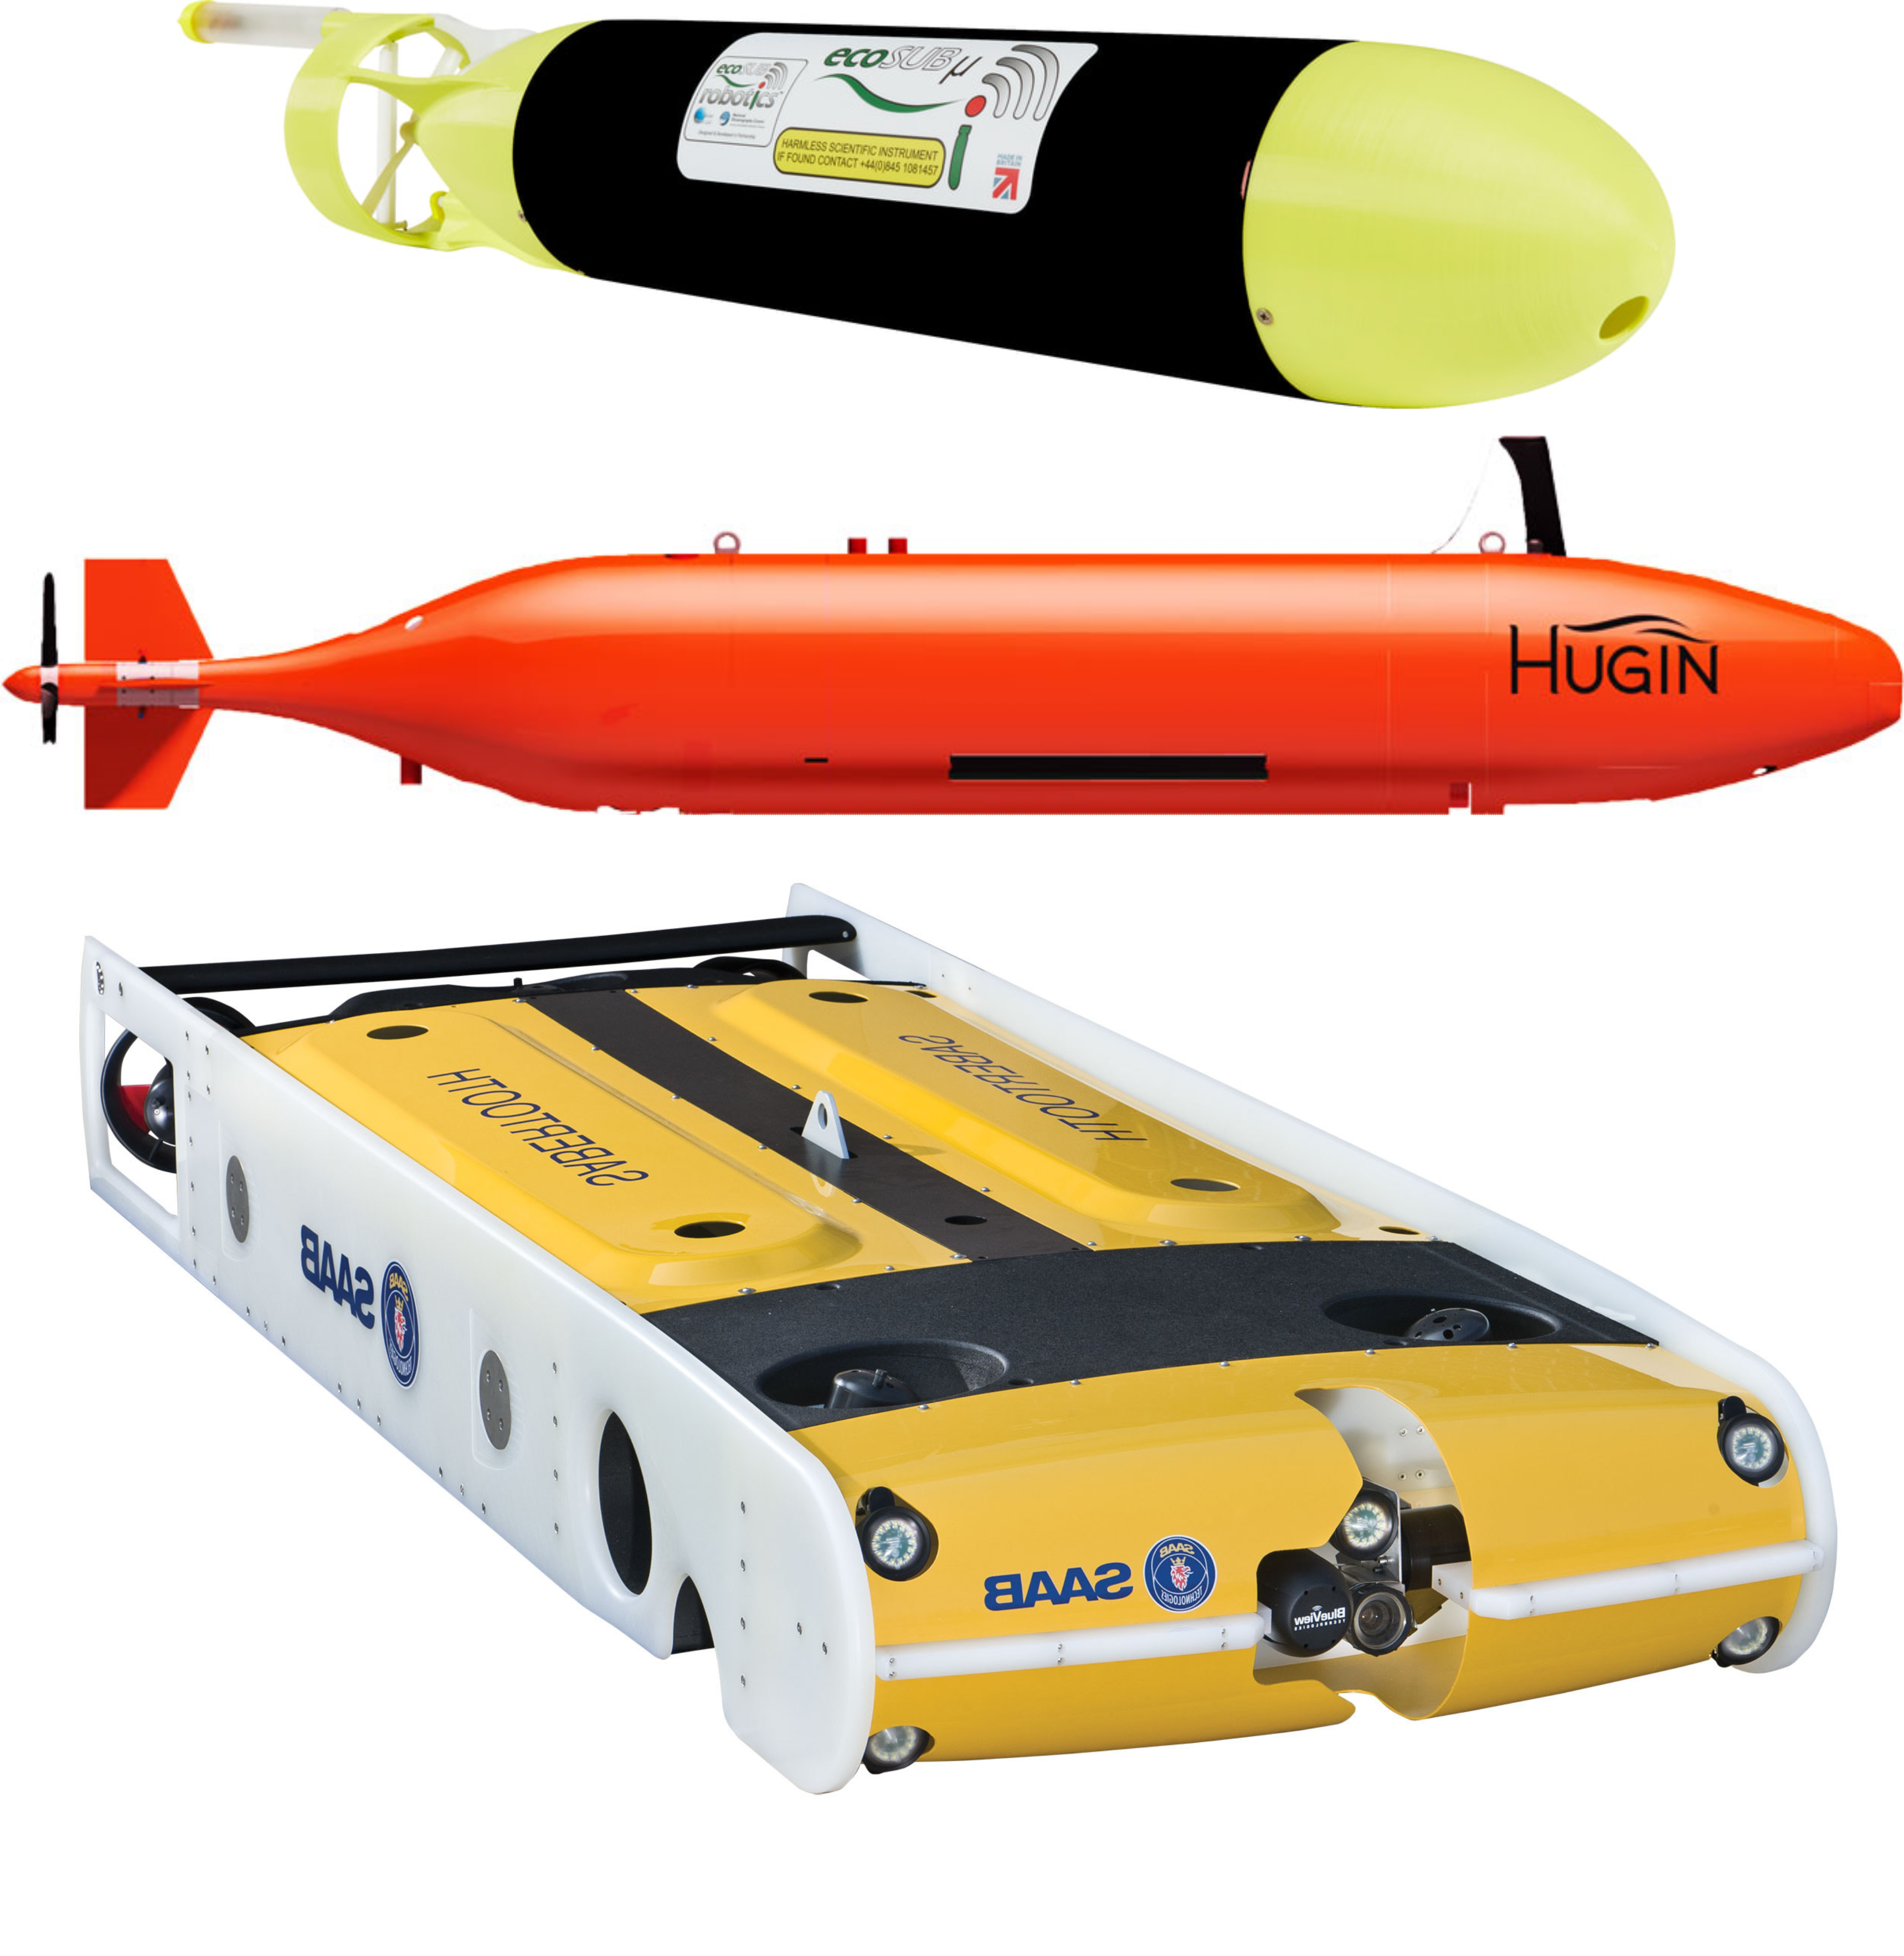
\includegraphics[width=0.5\textwidth]{figures/auvs2.png}
    \caption{Three \acrshort{auv}s; ecoSUB$\upmu5$ (Micro) \acrshort{auv}, Kongsberg Hugin survey grade \acrshort{auv}, and Saab Seaeye Sabertooth endurance \acrshort{auv}. The vehicles in the figure are not to scale relative to each other. }
    \label{fig:auvs}
\end{figure}

The \acrshort{auv} is a energy-constrained vehicle, usually running on batteries. As a rule of thumb, the \acrshort{auv} uses $2/3$ of its energy on propulsion and $1/3$ on the "hotel load", consisting of on-board computers and sensors. From hydrodynamics, the pressure-drag on a body moving through a liquid is proportional to the velocity squared. The power needed is then proportional to the velocity cubed, as $P=F\cdot v$, leading to a fairly hard upper limit of \acrshort{auv} speed of around $2.5$m/s. When designing an \acrshort{auv}, it is usually optimized for range, rather than speed, and depending on the hotel load, the optimal speed usually lies between 1 and 2 m/s. Depending on operating speed and available on-board energy, the endurance of an \acrshort{auv} can range from a few hours, as in the case of the Eelume, up to weeks in the case of Kongsberg Hugin Endurance. Gliders can have an endurance of months, being optimized for long-term deployments with low-power propulsion and payloads. 

\subsubsection*{Navigation}

It is hard to know where you are underwater, there is no GPS, and a submerged robot must rely on its on board systems and acoustic positioning systems to know where it is. Without acoustics, the drift of vehicles traversing underwater can be over $10\%$ of distance traveled, depending on the system. This adds an unknown noise to the measurements, it is unknown exactly \textit{where} the measurement is made. For seabed mapping, this uncertainty is quite familiar, and one of their main challenges, but in adaptive sampling it is usually ignored and interpreted as process or measurement noise. In the work reviewed and presented here, the navigation of the underwater vehicle has been assumed to be perfect, often motivated by frequent surfacing events such as in \textcite{fossum2021adaptive}, bounding the error. If one was to include the navigation uncertainty, one could modify the data sensing model as in Equation \eqref{eq:sense_alt} as an alternative to \eqref{eq:mod_meas}. 

\begin{align}
    \label{eq:sense_alt}
    y = f(\mathbf{x}+\mathbf{\varepsilon_x}) + \varepsilon
\end{align}

This formulation not found in the literature reviewed, but the noise can be interpreted as measurement or process noise, also known as the nugget. As long as the scale of the features measured is larger than the navigation uncertainty, it is usually ignored, and for open-ocean measurements, some hundred meters accuracy is sufficient. 


\subsubsection{Capabilities}
The propelled \acrshort{auv} is usually quipped for one of two purposes: 1) water column or 2) seabed mapping. In both cases, measurements are collected from the on-board sensors \textit{in-situ}. \acrshort{auv}s usually do not collect physical samples, with the notable exceptions of the third generation Environmental Sample Processor, mounted on a \acrfull{lrauv} \cite{pargett2015development} and the Dorado \acrshort{auv}  equipped with 10 2-liter water samplers (“gulpers”) \cite{zhang2011peak}. 

\section{Deterministic path planning}
Its quite good already
\subsection{Coverage}
\subsection{Monitoring}
\subsection{Drawbacks}
